\begin{figure}
	\centering
	\subfigure[$\delta t$ = 1 día]{
	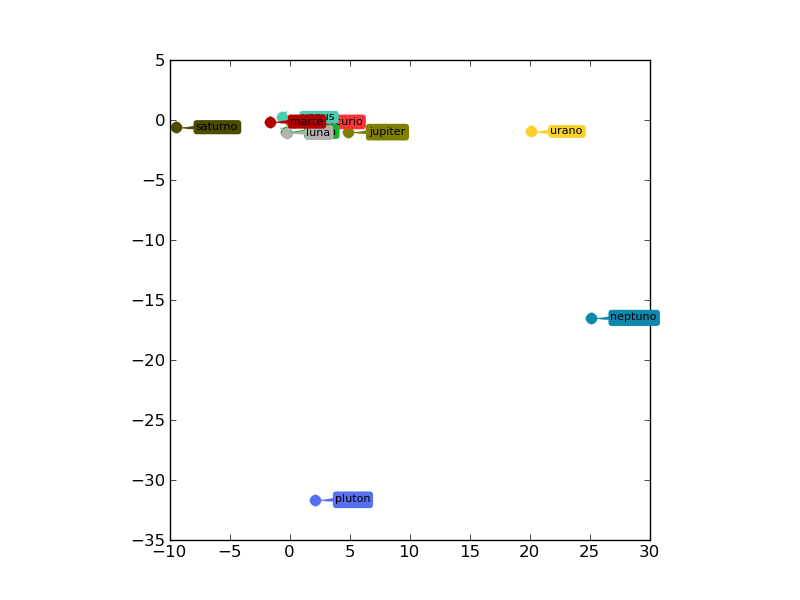
\includegraphics[scale=0.38]{img/ej2/metodo_2/validacion_30_1.png}
	\label{fig:ej2_m2_30_1}
	}
	\subfigure[$\delta t$ = 6 horas]{
	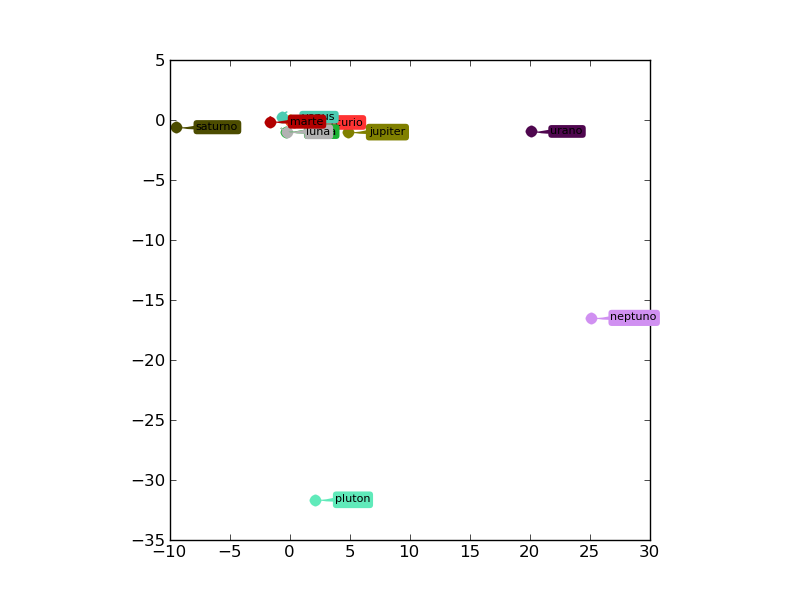
\includegraphics[scale=0.38]{img/ej2/metodo_2/validacion_30_4.png}
	\label{fig:ej2_m2_30_4}
	}
	\\
	\subfigure[$\delta t$ = 2 horas]{
	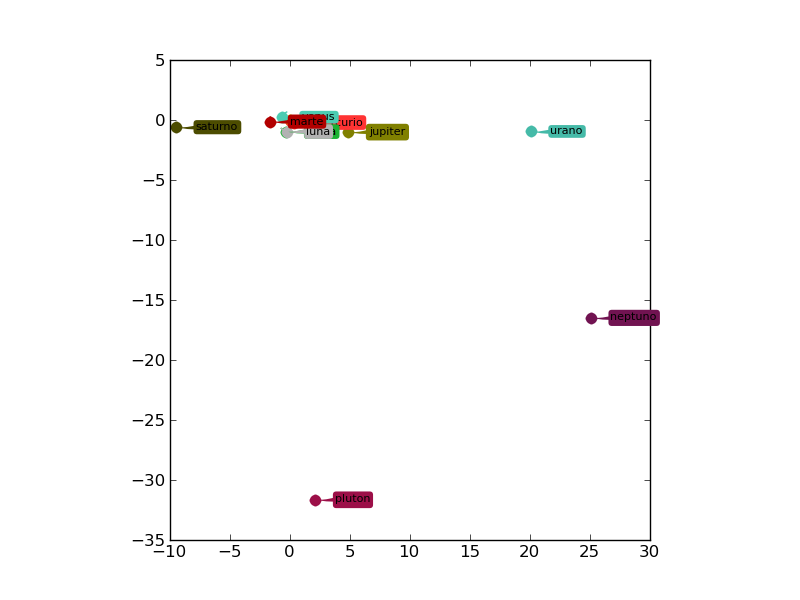
\includegraphics[scale=0.38]{img/ej2/metodo_2/validacion_30_12.png}
	\label{fig:ej2_m2_30_12}
	}
	\subfigure[$\delta t$ = 1 hora]{
	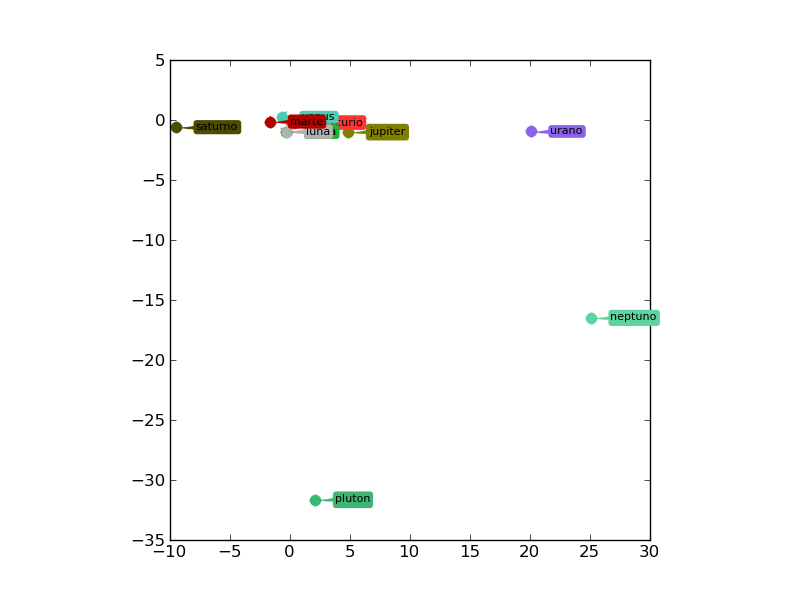
\includegraphics[scale=0.38]{img/ej2/metodo_2/validacion_30_24.png}
	\label{fig:ej2_m2_30_24}
	}
	\caption{
		Simulación de validación del sistema solar para un período de 30 días y distintos $\delta t$
		con el método 2.
		Observamos que el error no parece ser tan grande a simple vista para este período.
	}
	\label{ fig:res_ej2_m2_30 }
\end{figure}
\begin{figure}
	\centering
	\subfigure[$\delta t$ = 1 día]{
	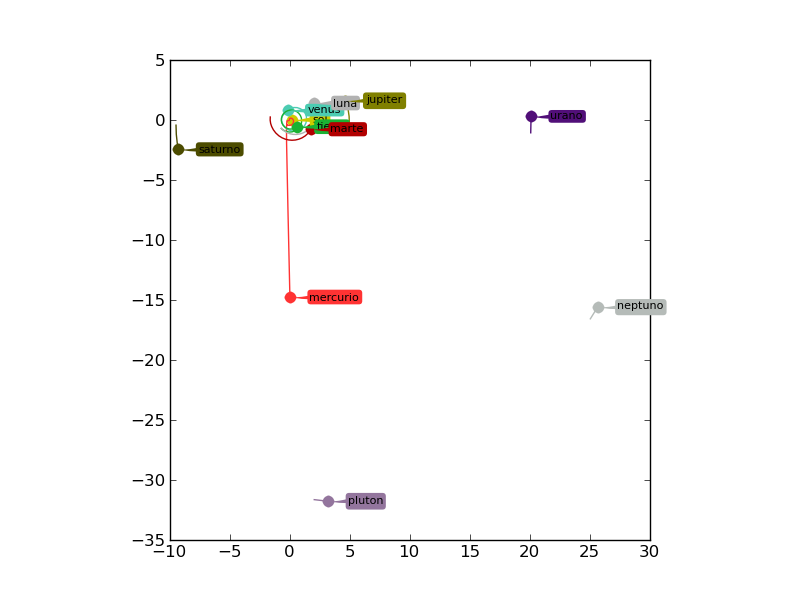
\includegraphics[scale=0.38]{img/ej2/metodo_2/validacion_365_1.png}
	\label{fig:ej2_m2_365_1}
	}
	\subfigure[$\delta t$ = 6 horas]{
	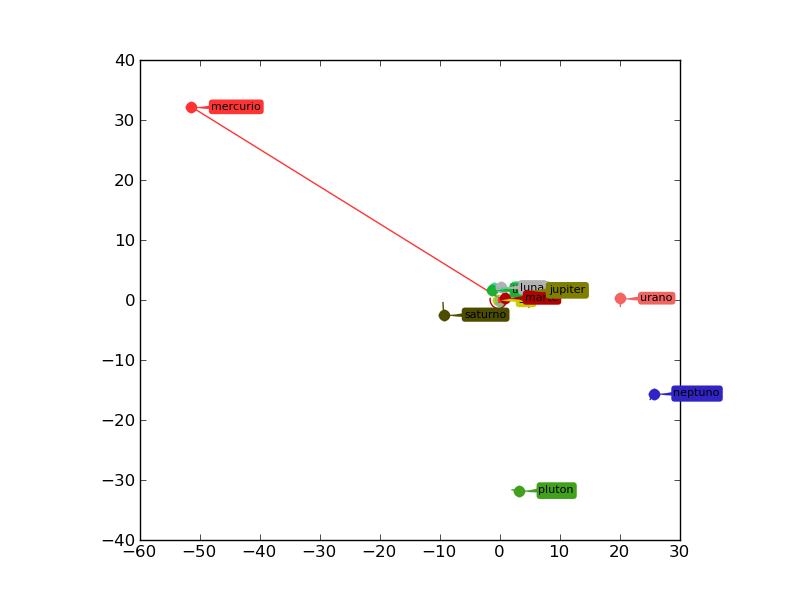
\includegraphics[scale=0.38]{img/ej2/metodo_2/validacion_365_4.png}
	\label{fig:ej2_m2_365_4}
	}
	\\
	\subfigure[$\delta t$ = 2 horas]{
	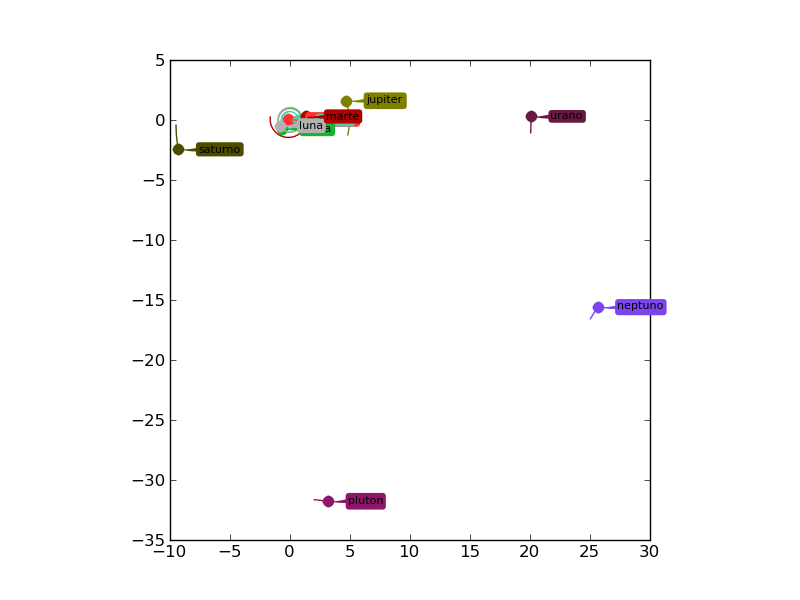
\includegraphics[scale=0.38]{img/ej2/metodo_2/validacion_365_12.png}
	\label{fig:ej2_m2_365_12}
	}
	\subfigure[$\delta t$ = 1 hora]{
	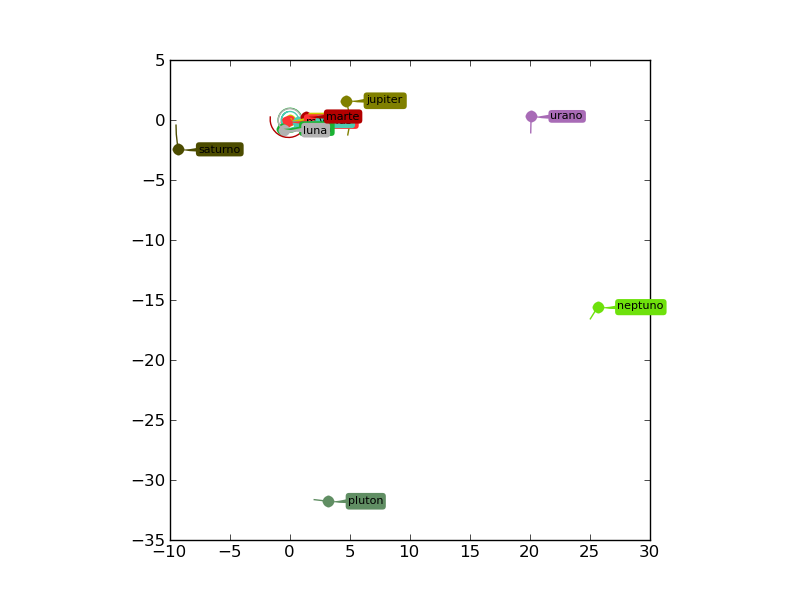
\includegraphics[scale=0.38]{img/ej2/metodo_2/validacion_365_24.png}
	\label{fig:ej2_m2_365_24}
	}
	\caption{
		Simulación de validación del sistema solar para un período de 1 año y distintos $\delta t$
		con el método 2.
		Para esta cantidad de tiempo, la simulación con un $\delta t$ de un día ya merece ser descartada.
		Las otras todavía parecen comportarse razonablemente
	}
	\label{ fig:res_ej2_m2_365 }
\end{figure}
\begin{figure}
	\centering
	\subfigure[$\delta t$ = 1 día]{
	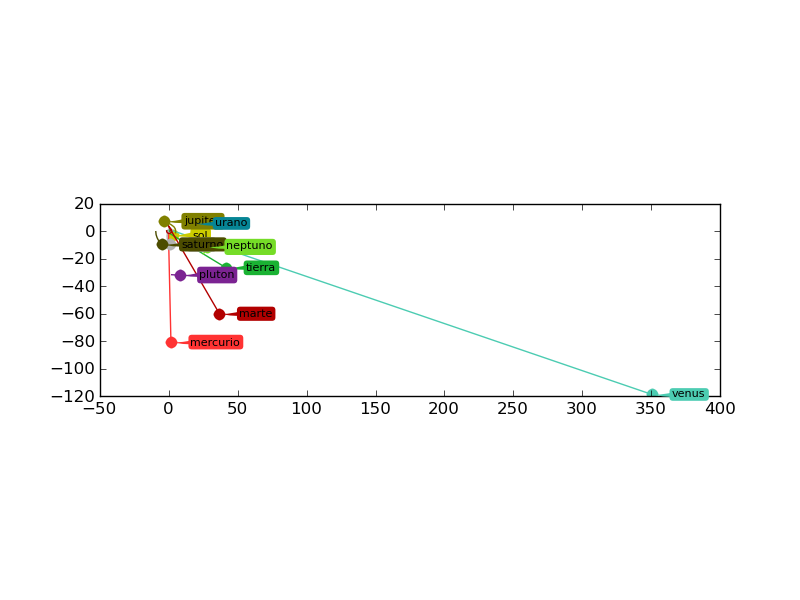
\includegraphics[scale=0.38]{img/ej2/metodo_2/validacion_1825_1.png}
	\label{fig:ej2_m2_1825_1}
	}
	\subfigure[$\delta t$ = 6 horas]{
	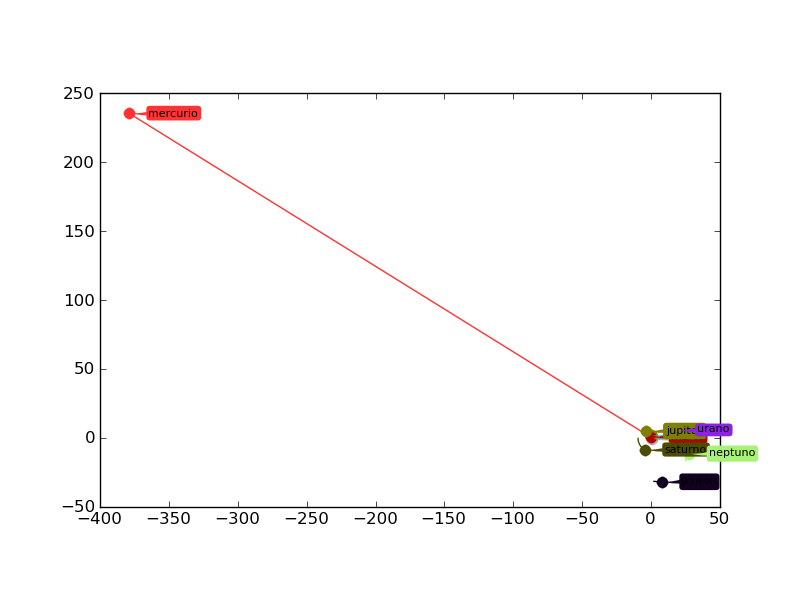
\includegraphics[scale=0.38]{img/ej2/metodo_2/validacion_1825_4.png}
	\label{fig:ej2_m2_1825_4}
	}
	\\
	\subfigure[$\delta t$ = 2 horas]{
	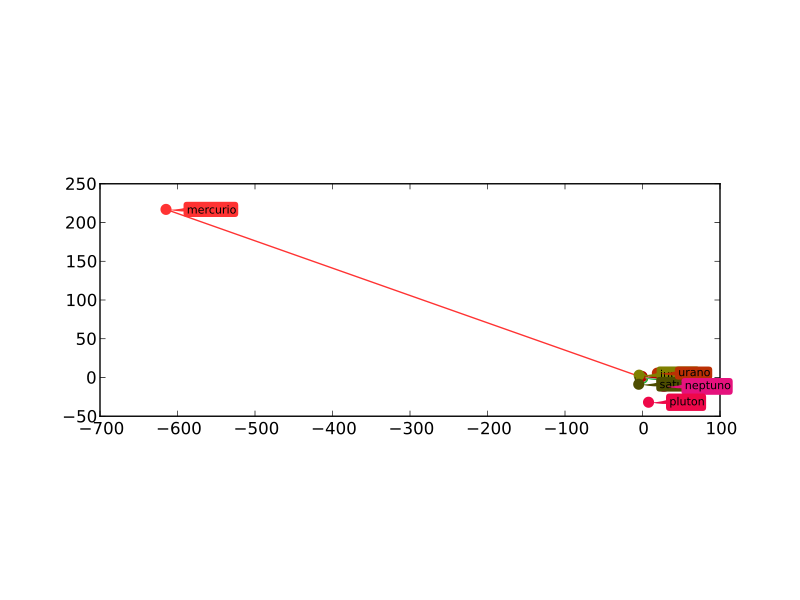
\includegraphics[scale=0.35]{img/ej2/metodo_2/validacion_1825_12.png}
	\label{fig:ej2_m2_1825_12}
	}
	\subfigure[$\delta t$ = 1 hora]{
	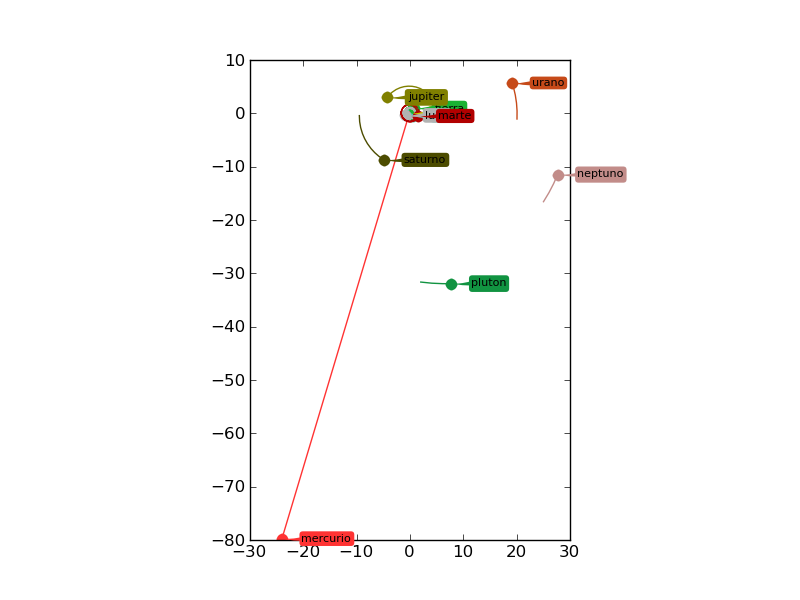
\includegraphics[scale=0.35]{img/ej2/metodo_2/validacion_1825_24.png}
	\label{fig:ej2_m2_1825_24}
	}
	\caption{
		Simulación de validación del sistema solar para un período de 5 años y distintos $\delta t$
		con el método 2.
		Para esta cantidad de tiempo de simulación, las órbitas de los planetas ya comienzan a mostrar error al dar más de una vuelta.
		El mejor método parece ser el de $\delta t$ de 2 horas, ya que para el de 1 hora la luna comienza a comportarse de una manera un poco mas extraña.
	}
	\label{ fig:res_ej2_m2_1825 }
\end{figure}
